
\fullcite{kemk13}

\begin{multicols}{2}
\begin{center}
{\bf Article excerpts}
\\ 
{\bf Notes and remarks}
\end{center}
\end{multicols}

%------------------------------------------------------------------------------

\begin{multicols}{2}
\includegraphics[width=8.4cm]{images/viscoelasticity/kemk13_a} \\
\[
\dot{\bm\varepsilon}^d = \frac{1}{2\eta} {\bm \tau}  + \frac{1}{2\mu} \check{\bm\tau} 
\]
The Jaumann objective derivative is used in order to account for 
stress rotation:
\[
\check{\bm \tau} = \frac{D{\bm \tau}}{Dt} 
- \dot{\bm \omega} \cdot {\bm \tau} + {\bm \tau} \cdot \dot{\bm\omega} 
\]
\[
\frac{D}{Dt} = \frac{\partial }{\partial t} + \vec\upnu \cdot \vec\nabla
\]
is the material derivative.

\end{multicols}

%------------------------------------------------------------------------------

\begin{multicols}{2}
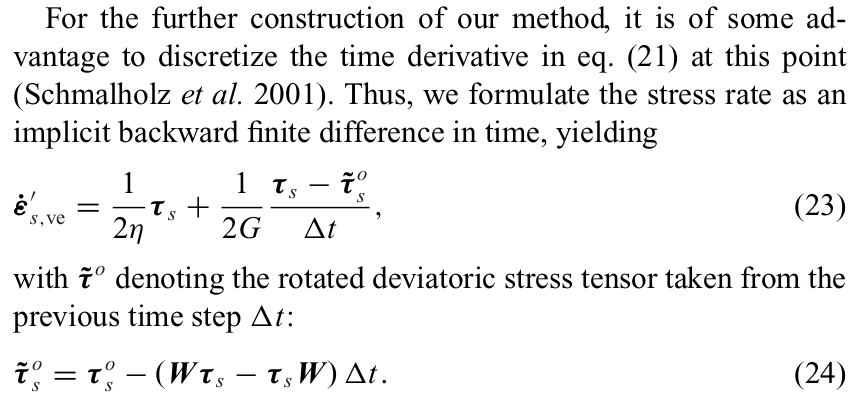
\includegraphics[width=8.4cm]{images/viscoelasticity/kemk13_b}
\end{multicols}

%------------------------------------------------------------------------------

\begin{multicols}{2}
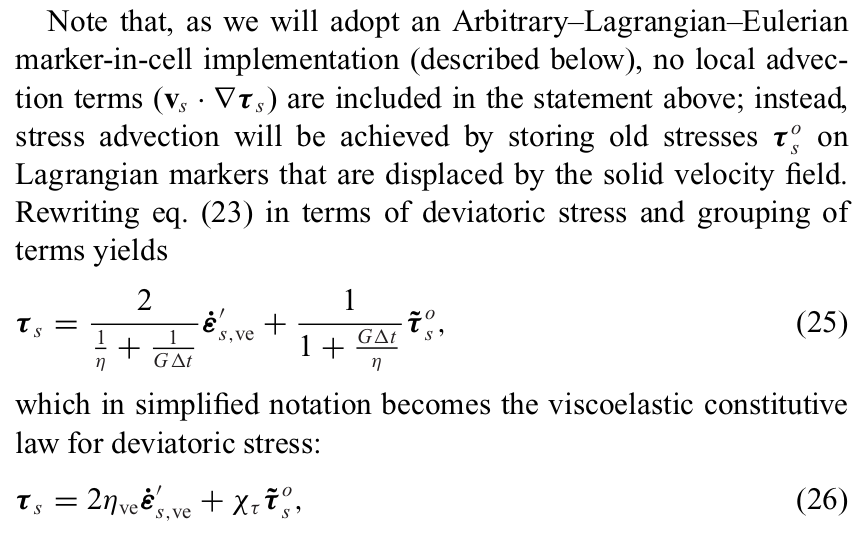
\includegraphics[width=8.4cm]{images/viscoelasticity/kemk13_c}
\end{multicols}

%------------------------------------------------------------------------------

\begin{multicols}{2}
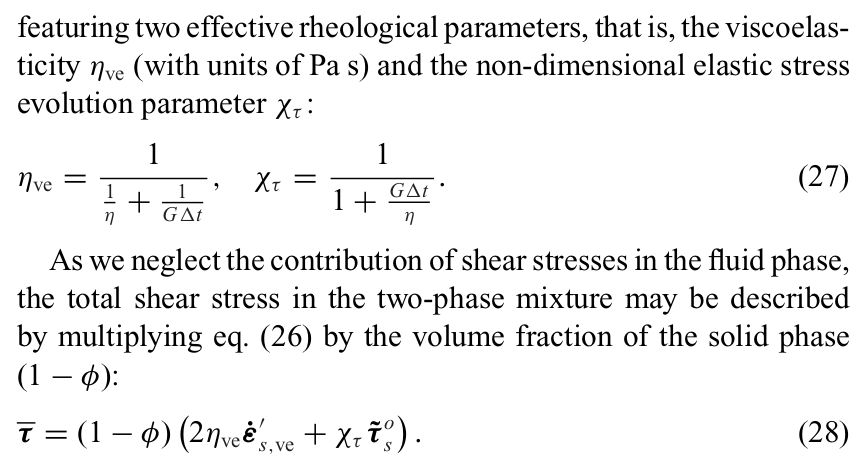
\includegraphics[width=8.4cm]{images/viscoelasticity/kemk13_d}
\end{multicols}

%------------------------------------------------------------------------------
